\documentclass{article}
\usepackage[margin=.9in]{geometry}              
\geometry{letterpaper}
\usepackage[parfill]{parskip}               
\usepackage{amssymb,amsmath}
\usepackage{amsthm}
\usepackage{mathtools}
\usepackage{enumerate}
\usepackage{gensymb}
\usepackage{tkz-graph}
\usepackage{tikz}
\usetikzlibrary{matrix}
\usepackage{cancel}
\usepackage[final]{pdfpages}


\usepackage[
backend=bibtex,
style=numeric,
citestyle=numeric,
maxbibnames=5,
sorting=none]{biblatex}

\bibliography{4f_pred} 

\makeatletter
\def\blx@maxline{77}
\makeatother


\graphicspath{{images/}}

\newenvironment{mycenter}[1][\topsep]
  {\setlength{\topsep}{#1}\par\kern\topsep\centering}% \begin{mycenter}[<len>]
  {\par\kern\topsep}% \end{mycenter}

\newenvironment{problem}{\rightskip1in}{\begin{mycenter}[-2pt]\rule{1.0\textwidth}{.4pt}\end{mycenter}}
 
\relpenalty=9999
\binoppenalty=9999

\theoremstyle{remark}
\newtheorem*{claim}{\\Claim}
\newtheorem*{lemma}{\\Lemma}
\newcommand{\inv}{^{-1}}
\newcommand{\pd}[2]{\frac{\partial #1}{\partial#2}}
\newcommand{\td}[2]{\frac{d#1}{d#2}}
\newcommand{\tab}{\hspace*{2em}}
\newcommand{\tn}[2]{\tensor{#1}{#2}}
\newcommand{\bp}[1]{\left(#1\right)}
\renewcommand{\t}[1]{\text{#1}}
\newcommand{\mb}[1]{\mathbb{#1}}
\newcommand{\mds}[1]{\mathds{#1}}
\newcommand{\mc}[1]{\mathcal{#1}}
\newcommand{\comp}[1]{\overline{#1}}
\newcommand{\AI}{A^{(4)}_{0|<I_{\t{in}}>}}
\newcommand{\lo}{\lambda_\t{opt}^{(4)}}
\newcommand{\ip}{$I\rightarrow P$ }

\linespread{1.25}
\renewcommand{\vec}[1]{\boldsymbol{#1}}
\newcommand{\horrule}[1]{\rule{\linewidth}{#1}}
\DeclarePairedDelimiter\abs{\lvert}{\rvert}%
\DeclarePairedDelimiter\ceil{\lceil}{\rceil}
\DeclarePairedDelimiter\floor{\lfloor}{\rfloor}

\title{HWPSS Prediction and Comparisons with POLARBEAR and EBEX}
\author{Jack Lashner, Joy Didier}




\begin{document}
\maketitle
\section*{Summary}
\tab In this memo we will explain our method of calculating the $n=4$ HWPSS, $\AI$. 
We will describe our current estimation for the polarized emission for the mirrors and $I\rightarrow P$ coefficients for the lenses. 
We will show our results for a standard optical chain, and also our results for the EBEX and POLARBEAR optical chains,
comparing with the measured HWPSS of those two experiments. 
\section*{Prediction}
\tab The dominating sources of polarized signal seen by the detector are polarized emission from the mirrors, and $I\rightarrow P$ leakage from windows and lenses.

\subsection*{Mirrors}
\tab From the Polarbear analysis \cite{takakura_performance_2017}  we can see that the IP leakage coefficient and the polarized emissivity of the mirrors are both given by
\[\lo(\nu, \chi) = 2 \sqrt{4 \pi \epsilon_0 \nu \rho} (\sec\chi - \cos\chi).\]
where $\rho = 2.417\times 10^{-8} \; \ohm \cdot \t{m}$ is the resistivity of the metal, and $\chi$ is the incident angle of the light.
Here we are including the factor of 2 in the Hagen-Rubens formula which gives a better fit to data.

\tab Our total polarized power from each mirror with incident angle $\chi$ will then be
\[
P^{p} = \int_{\nu_\t{low}}^{\nu_\t{high}} \lo(\nu, \chi) B(\nu, 300 \t{ K}) d\nu.
\]


\tab For the time being we are ignoring the curvature of the mirrors, and using the geometry specified in the CCAT optical design document.
This gives us average incident angles of $\chi = 25.73 \degree$ for the primary mirror, and $\chi = 19.59\degree$ for the secondary mirror.
\subsection*{Lenses}
\tab To estimate the $I\rightarrow P$ coefficients we use data gathered by Brian Koopman for the ACTPol telescope, by propagating unpolarized light throught the system until it reached the detector array using Code V. 
This is data shown in Figure \ref{fig:IP-array}. 
We can see that the \ip varies from .12\% on the edge of the array to less than .015\% towards the center.
This simulation only takes into account the contribution for the lenses (of which there are three), so for each lens we simply dividing the total \ip by 3, which gives us .04\% and .005\% for the edge and center respectively.

\begin{figure}[t!]
	\centering
  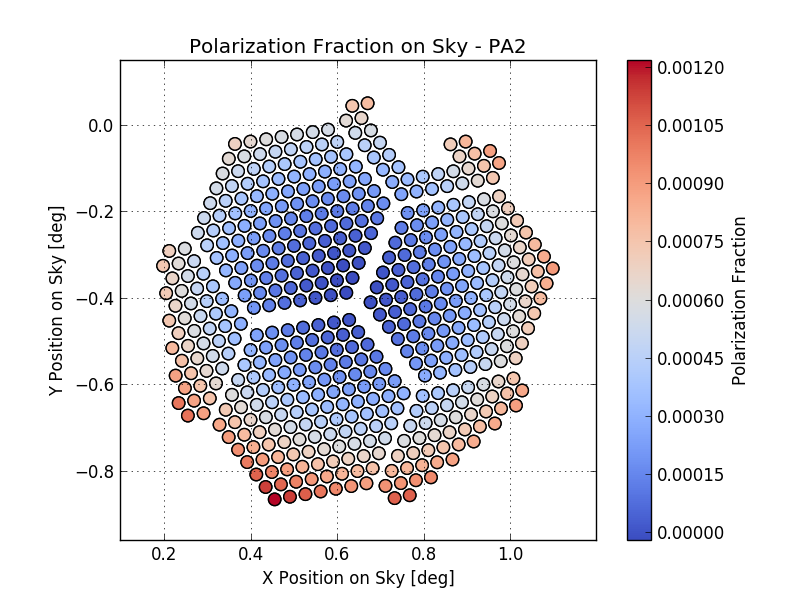
\includegraphics[width=.8\linewidth]{images/pa2_polarization_fraction.png}
  \caption{$I\rightarrow P$ coefficients due to lenses across the detector array of ACTPol.}
  \label{fig:IP-array}
\end{figure}

\subsection*{Filters}
\tab Though it is not currently included in our calculation, it is also necessary to consider \ip coming from the mesh filters. 
The $s$ and $p$ transmission of our filters are given in \cite{pisano_polarisation_2006} for incident angles of 
$\chi = 0\degree \t{ and } \chi = 15\degree$ for frequencies above 150 GHz.
From the paper alone, we are able to see that the $s$ and $p$ transmissions are indistinguishable at 0\degree, 
and at 15\degree the maximum \ip in our desired frequency range is about .1\%.

\tab This is much more than we actually expect, since the maximum incident angle in our current optical setup is 
around 7.5\degree, and this only occurs at the very edges of the beam.

Additional work is required to come up with a more realistic upper bound on the \ip.


\subsection*{Propagation}
\tab Using this information we may propagate the power through each element.
In this first iteration, if $P_{n}^{u/p}(\nu)$ is the unpolarized / polarized incident power on the $n^\t{th}$ optical element, 
we calculate the incident power on the $(n+1)^\t{th}$ element as
\begin{align}
P_{n+1}^u(\nu) &= P_n^u(\nu) \eta_n^u(\nu) (1 - \eta_n^{\t{ip}}(\nu)) + A\Omega(\nu) \; \varepsilon_n^u(\nu) B(\nu,T_n)\\
P_{n+1}^p(\nu) &= P_n^u(\nu) \eta_n^u(\nu) \eta_n^{\t{ip}}(\nu) +  P_n^p(\nu) \eta_n^p(\nu) + A\Omega(\nu) \; \varepsilon_n^p(\nu) B(\nu,T_n)
\end{align}
where $\eta_n^{u/p}$ is the unpolarized/polarized efficiency of element $n$, $\eta_n^\t{ip}$ is the \ip coefficient, $\varepsilon_n^{u/p}$
is the unpolarized/polarized emissivity, and $B(\nu,T)$ is the spectral brightness.

\tab The absorption and reflection coefficients are given in the optical chain file and shown in Table 
\ref{table:SO_OpticalChain}. Additional info such as scattering and spillover coefficients are also given.
Because elements are in thermal equilibrium, the absorption is equal to the emissivity $\varepsilon$.
The only exception to this is the primary mirror, where spillover onto heated surfaces adds additional emissivity.
The efficiency $\eta$ is then given by subtracting each coefficient from 1:
\[\eta_n = 1 - \t{abs}_n - \t{refl}_n - \t{scatt}_n\]

\tab After the HWP, additional polarized signal no long contributes to our measurement, 
so the propagation of the polarized power simply becomes
\begin{align}
P_{n+1}^p(\nu) &=  P_n^p(\nu) \eta_n^p(\nu) 
\end{align}


To get the total unpolarized/polarized power on the detector we integrate 
\[
P^{u} = \frac{1}{2}\int_{\nu_\t{low}}^{\nu_\t{high}} P_\t{det}^u(\nu) d\nu,
\qquad \qquad
P^{p} = \int_{\nu_\t{low}}^{\nu_\t{high}} P_\t{det}^p(\nu) d\nu
\]
$P_\t{det}$ is the power once the efficiency of the detector is already taken into account. 
$A\Omega$ is already accounted for in the propagation.
The factor of 1/2 is needed when calculating the unpolarized power because we are measuring a single linear polarization,
while it is not included in the polarized power since we do not know the orientation of the polarization of the incoming light, 
and are looking for the maximum value.

\section*{Results}
\tab Since these calculations are very similar to those done in Charlie Hill's sensitivity code,
our code was built to be compatible with his input files.
We have run the model with the input data for the 45 cm aperture and silicon lenses for various HWP positions:
between the first lense and the window, between the second and first lenses, and between the 2nd lens and the aperture.
The optical chain and HWP positions are shown in Table \ref{table:SO_OpticalChain}.
The HWPSS seen by the detector for each HWP position is shown in Table \ref{table:SO_powers}.


\begin{table}
\begin{center}

\begin{tabular}{ |l|c|c|c|c|} 
	\hline
	\multicolumn{5}{|c|}{SO Optical chain}\\
	\hline
	 Name 		& Temp (K)	& Abs (150 GHz) & Abs (250 GHz) & Reflection \\ \hline
	 Mirror 	&	273		& 0.002 & .005 & 0 \\
	 \hline \multicolumn{5}{|c|}{POLARBEAR HWP }\\ \hline
	 Mirror 	&	273		& 0.002 & .005 & 0 \\
	 Window 	&	265		& 0.005 & .010 & 0.01 \\
	 \hline \multicolumn{5}{|c|}{HWP pos 1 (80 K)}\\ \hline
	 IRShaders 	&	80		& 0.001 & .001 & 0 \\
	 IRShaders 	&	40		& 0.001 & .001 & 0 \\
	 LowPass 	&	10		& 0.010 & .010 & 0.05 \\
	 Lens 		&	4.5		& 0.007 & .011 & 0.006 \\
	 \hline \multicolumn{5}{|c|}{HWP pos 2 (4 K)}\\ \hline
	 Lens 		&	1.2		& 0.007 & .011 & 0.006 \\
	 \hline \multicolumn{5}{|c|}{HWP pos 3 (4 K?)}\\ \hline
	 Aperture 	&	1.2		&  NA  &  NA  & NA \\
	 Lens 		&	1.2		& 0.007 & .011 & 0.006 \\
	 LowPass 	&	1.2		& 0.010 & .010 & 0.050 \\
	 LowPass 	&	1.2		& 0.010 & .010 & 0.050 \\
	 LowPass 	&	.1		& 0.010 & .010 & 0.050 \\
	\hline	
\end{tabular}
\end{center}
\caption{Our current optical chain with a 45 cm aperture and silicon lenses.
Shown is also the three HWP positions which we have considered, and the HWP position used for our POLARBEAR comparison.
}

\label{table:SO_OpticalChain}
\end{table}



\begin{table}
\centering

\begin{tabular}{ |c|c|c|c| } 
	\hline
	 & \multicolumn{3}{|c|}{HWPSS (pW)}\\
	\hline
	freq(GHz) & pos 1 	& pos 2 & pos 3 \\ \hline
	27  & .00057, .00057 & .00063, .00058 & .0007, .00059 \\
	39  & .00253, .00253 & .00289, .00257 & .00326, .00262	 \\
	93  & .00766, .00766 & .00849, .00776 & .00932, .00787 	 \\
	145 & .01880, .01899  & .02076, .01912   & .02262, .01936 	 \\
	233 & .05883, .05883   & .06671, .05981   & .0746, .0608 	 \\
	\hline	
\end{tabular}


\begin{tabular}{ |c|c|c|c| } 
	\hline
	 & \multicolumn{3}{|c|}{HWPSS (K$_\t{CMB}$)}\\
	\hline
	freq (GHz) & pos 1 	& pos 2 & pos 3 \\ \hline
	27  & .07139, .07139 	 & .07930, .07238 & .0872, .07337 \\
	39  & .08735, .08735 & .09993, .08892 & .1125, .09049	 \\
	93  & .16139, .16139 & .17955, .16413 & .19719, .16634 	 \\
	145 & .27242, .27242  & .2993, .27579   & .3262, .27916 	 \\
	233 & .70232, .70232   & .796, .71409   & .8906, .72586 	 \\
	\hline	
\end{tabular}


\caption{ Calculated $\AI$ for the optical chain in table \ref{table:SO_OpticalChain} at the three positions shown.
In each cell, the first number is $\AI$ for a detector towards the edge of the array, and the second number 
is for a detector towards the center. We present the power in both pW and K$_\t{CMB}$
}
\label{table:SO_powers}
\end{table}




\section*{Comparisons}

\tab In order to test the credibility of our results we tested our method with optical setups resembling those of POLARBEAR and EBEX,
and compared our results to their predicted results, and measured results. 

\subsection*{POLARBEAR}
\tab For a simplified comparison, we used the same optical chain as SO, but with a HWP in between the first and second mirrors.
For the primary mirror we use 32.5\degree, as stated in \cite{takakura_performance_2017}. At $\nu = 145 \t{ GHz}$ this gives us a final 
HWPPS of $\AI = .029175 \t{ pW}$. Using the conversion $\eta = .18 \t{ pW/K}$, this give us 162 mK.
This is consistent with the average measurements given in Table 1 of \cite{takakura_performance_2017}, which is about 160 mK.

\subsection*{EBEX}

\tab For our comparison with EBEX we use the optical chain given in Christopher Geach's memo on May 1st.
In his analysis Christopher calculates the average polarization fraction across the curved mirror
\[p(\chi) = \frac{\sin^2 \chi}{1 + \cos^2 \chi}\]
to be 15.6\% for the primary mirror and 6.4\% for the secondary mirror. 
We then solve for $\chi$ to be used in our own calculations, which gives us $31.3\degree$ and $20.3 \degree$.
At 150 GHz, the \ip of the field lens is about 2.7\% towards the edge of the array.
Using these values we end up with $\AI = .2218 \t{ pW}$, which is larger than their observed value of 0.158 pW.

\tab A possible reason for this is because 2.7\% is the maximum \ip value throughout the detector. 
Decreasing this coefficient to 1.7\% gives us $\AI = .154 \t{ pW}$ which is much closer to the measured result.





\printbibliography


\end{document}

